\section{实验背景}

\frame{\frametitle{流场显示实验溯源及应用}
\begin{columns}
\begin{column}[c]{0.4\textwidth}
\begin{center}
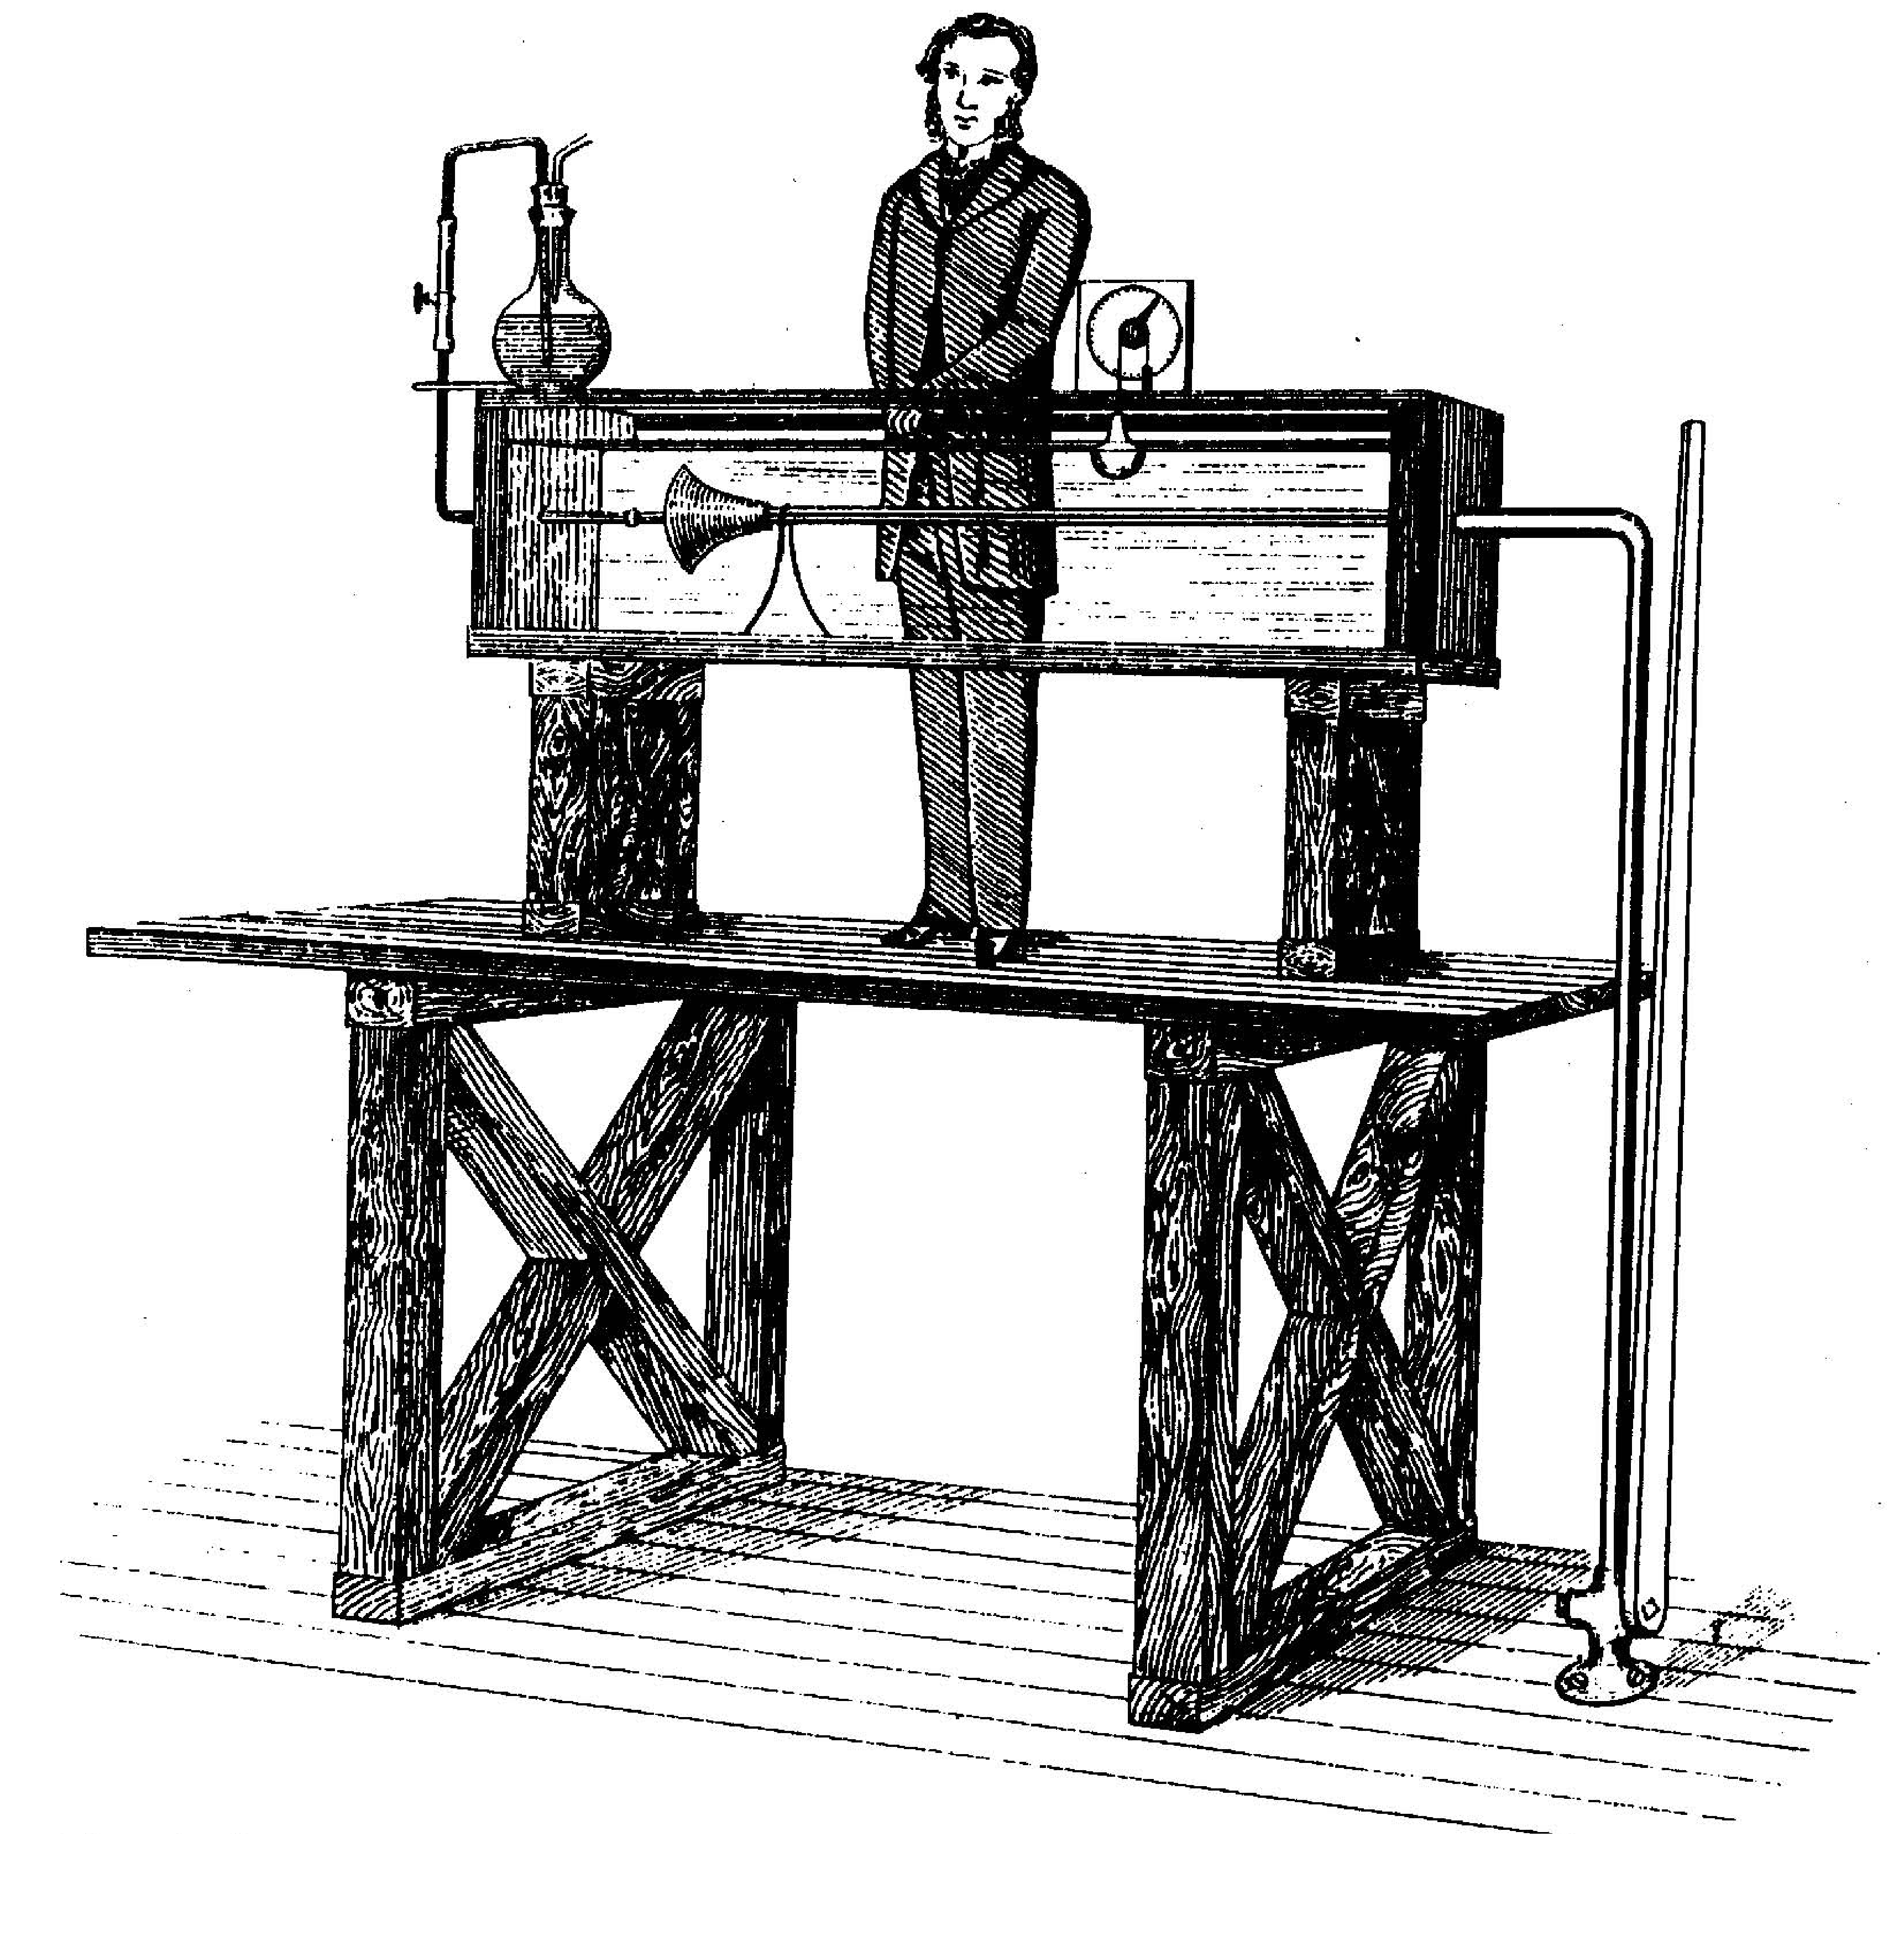
\includegraphics[width=1\textwidth]{Reynold.pdf}
\end{center}
\end{column}
\begin{column}[l]{0.6\textwidth}
\begin{itemize}
\item 流场显示实验可以追溯到1883年雷诺的流场显示实验.
\item 自雷诺实验后, 这门技术的原理性和技术性文献不断涌现, 形成了一门独特的实验技术科学.
\item 流场显示技术已被广泛应用于流体力学、空气动力学、爆炸力学、等离子体物理、燃烧学、传热学、核子物理等一系列领域中.
\end{itemize}
\end{column}
\end{columns}
}

\frame{\frametitle{常用流场显示技术}
常用流场显示技术有:
\begin{itemize}
\item \textbf{外加物质法}: 在透明无色的气流或水流中加入一些可见的粒子, 通过可见的外加粒子跟随流体微团的运动来使各种流动现象显示出来.(氢气泡, 染料溶液等)
\item \textbf{注入能量法}: 将能量加到流场中的部分流体上, 使它们的某些性质(如密度, 辐射能)与其它部分的流体区别开来, 以便用光学方法加以观察和记录. 加入能量的方式有电热丝加热, 电极放电, 激光聚焦, 电子束等.
\item \textbf{光学方法}: 利用流场的光学性质, 如气体的光学折射率是其密度的函数, 通过流场的折射率变化来显示某些流动现象, 通常用于高速流场中.
\end{itemize}
}

